\clearpage
\section{Tests and verification}

Described in this section is a test suite intended to verify that the designed
hardware, firmware and software behave correctly and meet project requirements.
Because the three components are heavily co-dependent, conducting pure unit
tests would require the development of dedicated simulation software. This has
not been done as part of the thesis; as such, this test suite depends on all
components functioning correctly at the same time.

\subsection{Hardware tests}

The hardware must:
\begin{enumerate}
    \item Support microcontroller operation when supplied with 12 volts
    \item Be programmable through ISP
    \item Establish communication over USB
    \item Drive all stepper motors correctly
\end{enumerate}

The prined circuit board presented in section~\ref{pcbsection} was set up as
shown in figure~\ref{pcbsetup}. Power was supplied from an benchtop power
supply. Current consumption on power-up was 30 mA and the transmit LED blinked
every quarter second, indicating that the microcontroller is functioning
properly and sending feedback.

\begin{figure}[ht]
    \centering
    \begin{minipage}{0.5\textwidth}
        \centering
        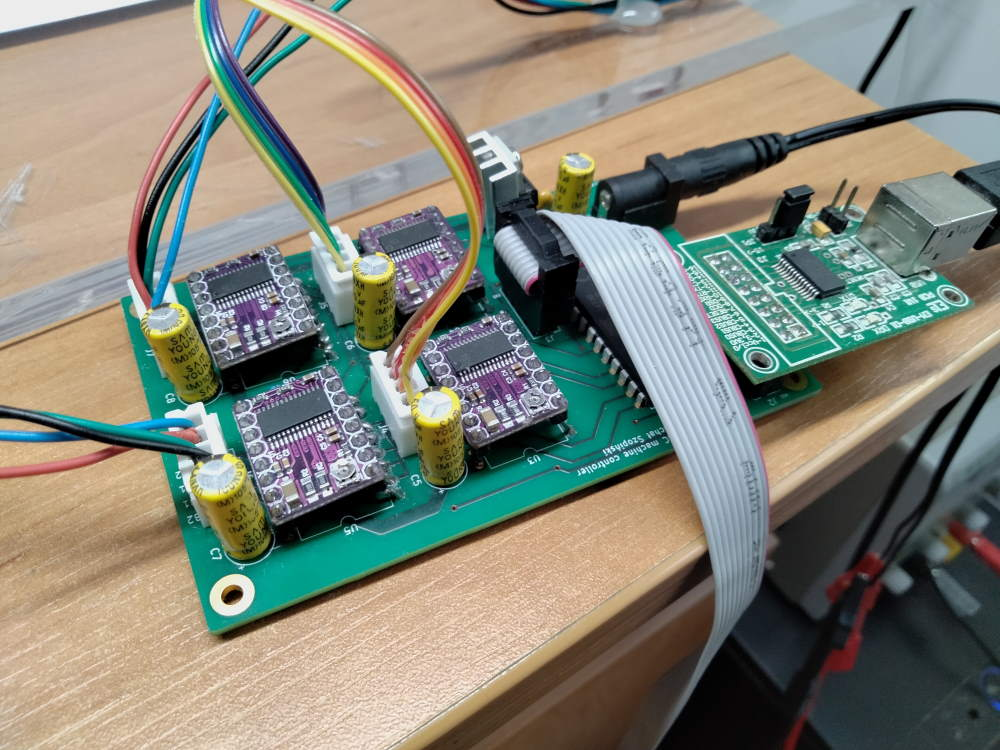
\includegraphics[width=0.9\textwidth]{pcbsetup}
        \caption{PCB set-up.}
        \label{pcbsetup}
    \end{minipage}\hfill
    \begin{minipage}{0.5\textwidth}
        \centering
        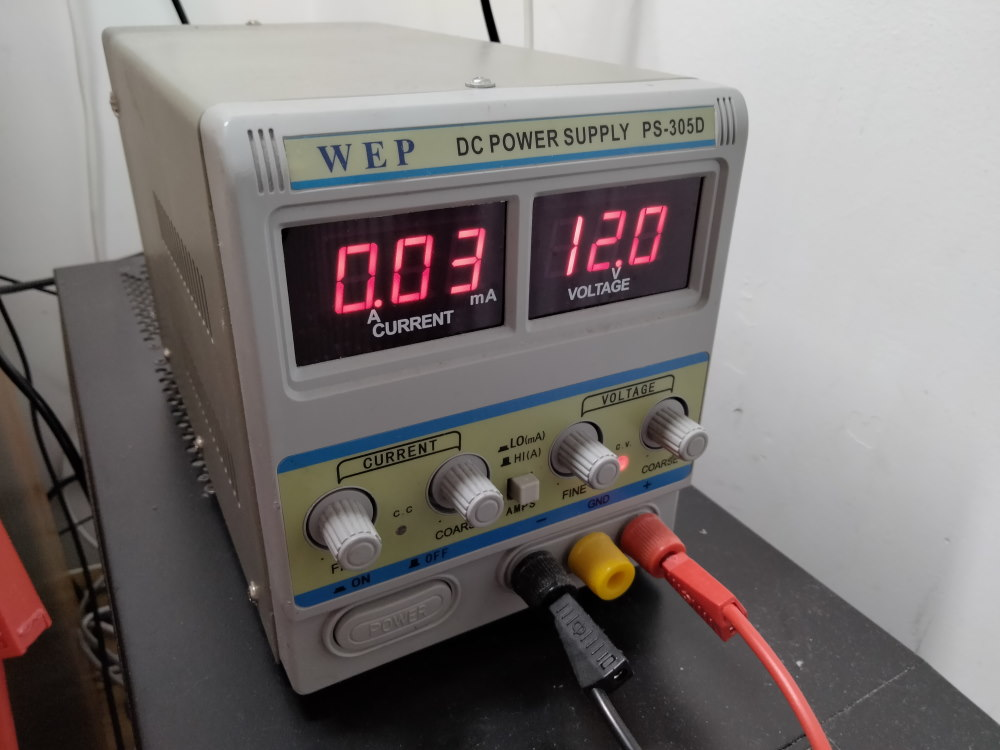
\includegraphics[width=0.9\textwidth]{current}
        \caption{Initial current consumption.}
        \label{current}
    \end{minipage}
\end{figure}

A USBasp programmer was connected to the ISP port to verify the device's
in-system programming capability. An attempt to upload the firmware binary was
successful. Opening the device's virtual serial port in a terminal emulator
revealed the structure of the periodically sent feedback
(figure~\ref{feedback}).

Issuing several \texttt{G0} commands initiated rapid movement. All motors were
driven correctly. The machine moved smoothly in all three axes.

\begin{figure}[ht]
    \begin{center}
        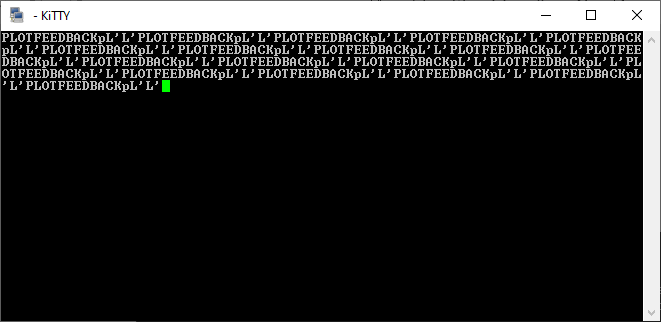
\includegraphics[width=0.6\textwidth]{feedback}
        \caption{Feedback data viewed in a terminal.}
        \label{feedback}
    \end{center}
\end{figure}

\subsection{Firmware tests}

Because the firmware issues feedback in a human-unreadable binary form, all
tests of the firmware were conducted through the control software's command
prompt. The software provides a way to inspect the received feedback and gain
insight into the way the firmware operates.

The firmware must:
\begin{enumerate}
    \item Read and parse commands
    \item Provide periodic feedback describing the machine's current position
    \item Provide feedback on the execution of commands, including their
    interpretation
    \item Handle and provide diagnostics for syntax and semantic errors in
    commands
    \item Support rapid, linear and arc motion
    \item Support commands for switching between absolute and relative
    coordinates
    \item Support commands for changing the units of measurement
\end{enumerate}

\subsubsection{Command parsing and feedback}

When the device was first powered on, periodic feedback was observed in the
terminal window. For the purpose of this test, the control software was modified
to display a human-readable representation of the feedback. The machine sent
data describing its position (figure~\ref{posfeedback}) and the interpretation
of commands it received (figure~\ref{comfeedback}).

\clearpage
\begin{figure}[ht]
    \centering
    \begin{minipage}{0.5\textwidth}
        \centering
        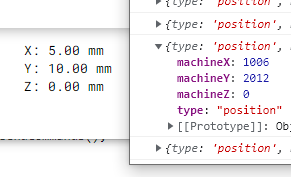
\includegraphics[width=0.9\textwidth]{positionfeedback}
        \caption{Position feedback, raw data and conversion to millimeters.}
        \label{posfeedback}
    \end{minipage}\hfill
    \begin{minipage}{0.5\textwidth}
        \centering
        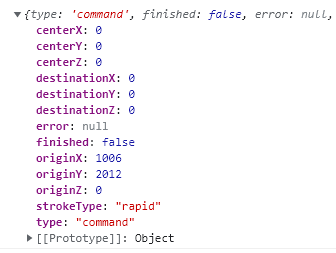
\includegraphics[width=0.9\textwidth]{commandfeedback}
        \caption{Command feedback.}
        \label{comfeedback}
    \end{minipage}
\end{figure}

The firmware's ability to parse and validate syntax was tested. Several commands
were issued testing various productions of the command language
(figure~\ref{syntax}). The parser correctly handles G-code words with decimals,
comments, command deletion and line number markers. Errors are reported when
the parser encounters syntax errors and unsupported features: parameter
settings, unimplemented word letters, unimplemented G-word numbers.

\begin{figure}[ht]
    \begin{center}
        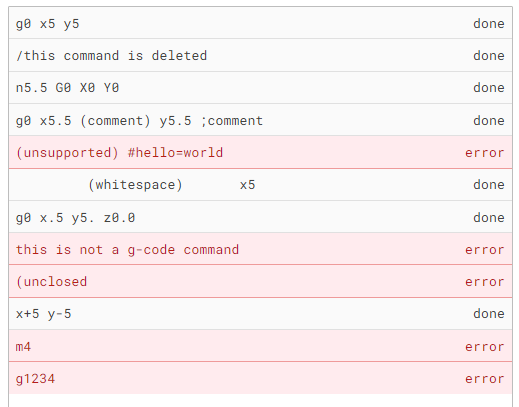
\includegraphics[width=0.6\textwidth]{syntax}
        \caption{Commands correctly parsed by the firmware.}
        \label{syntax}
    \end{center}
\end{figure}

\subsubsection{Command execution}

Two G-code files were prepared to demonstrate the machine's ability to execute
rapid, linear and arc movement. The machine successfully executed the commands
and drew geometric patterns on paper (figure~\ref{lineararc}). A series of
commands was prepared to test modal G-codes. The machine behaved as intended
(figure~\ref{modals}).

\begin{figure}[ht]
    \begin{center}
        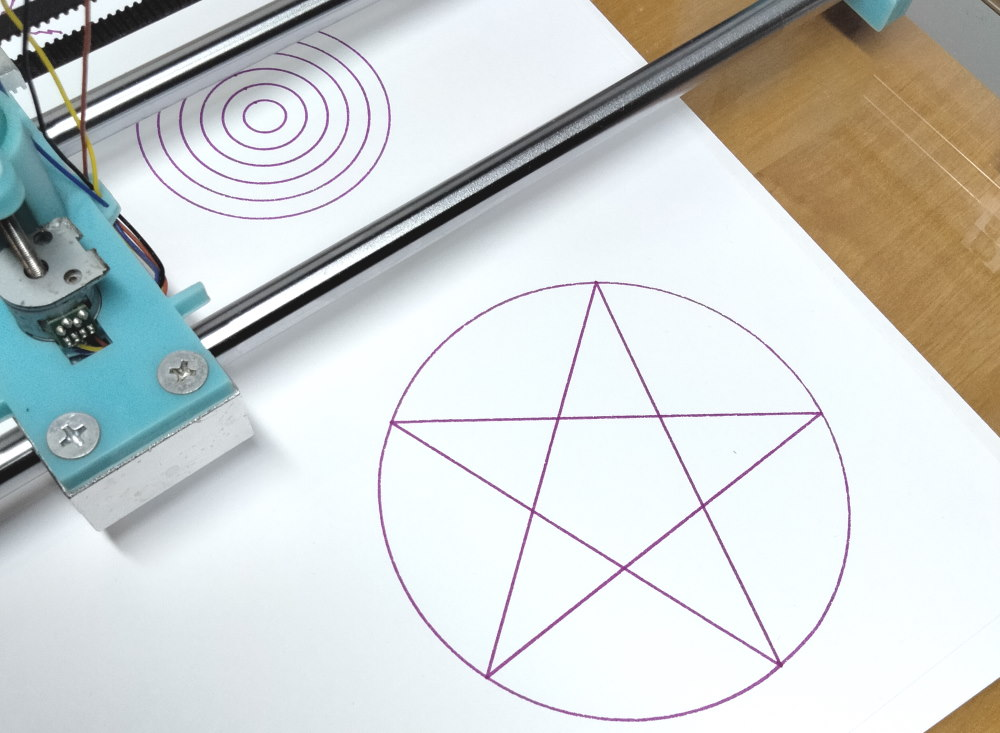
\includegraphics[width=0.8\textwidth]{lineararc}
        \caption{Lines and arcs drawn by the machine.}
        \label{lineararc}
    \end{center}
\end{figure}

\begin{figure}[ht]
    \begin{center}
        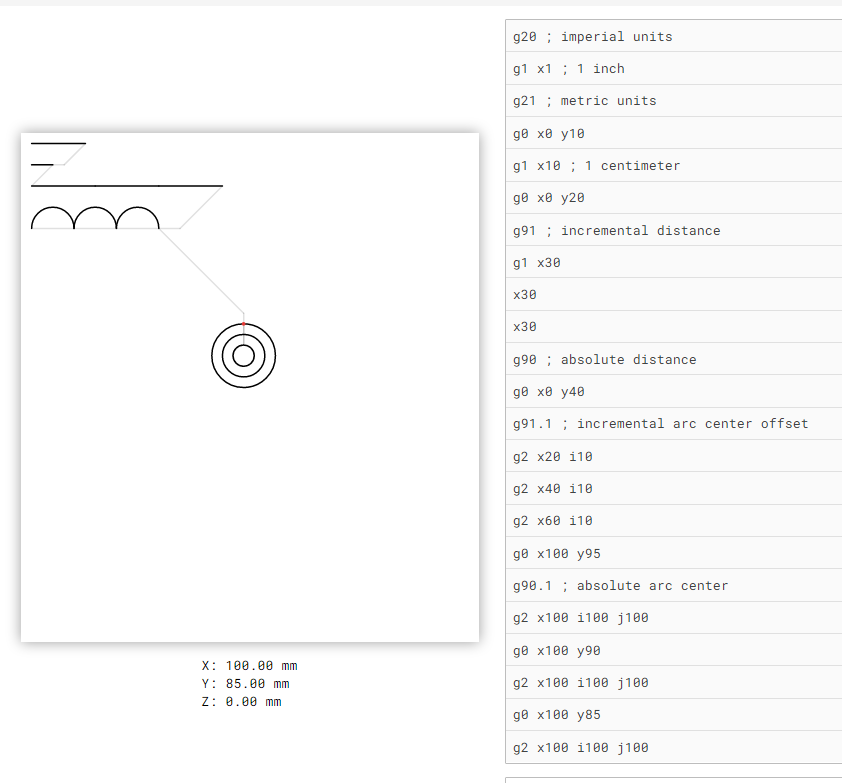
\includegraphics[width=0.8\textwidth]{modal}
        \caption{Modal commands and their impact on command execution. Preview
        drawn based on interpretation data from the machine.}
        \label{modals}
    \end{center}
\end{figure}

\clearpage
\subsection{Software tests}

The software's ability to perform basic tasks (connect to the machine,
send and receive commands) has largely been verified in the previous sections.
This section verifies the remaining major components of the user experience.

The software must be able to:
\begin{itemize}
    \item Establish connections and handle connection errors
    \item Keep track of sent commands and display feedback to the user
    \item Generate a preview of motion initiated by the commands
    \item Trace bitmaps
\end{itemize}

\subsubsection{Connectivity}

When the application is launched, the user is presented with a serial port
selection screen. Selecting a port prompts an attempt to establish a connection.
The machine has been verified to correctly handle the following error
conditions:
\begin{enumerate}
    \item Connection failures -- verified by disconnecting the device's power
    supply
    \item Feedback timeouts -- verified by holding the microcontroller in reset
    state
    \item Malformed feedback -- verified by resetting the microcontroller
    mid-transmission
\end{enumerate}
An error dialog is displayed and the software returns to the port selection
screen (figure~\ref{connfailed}).

\begin{figure}[ht]
    \begin{center}
        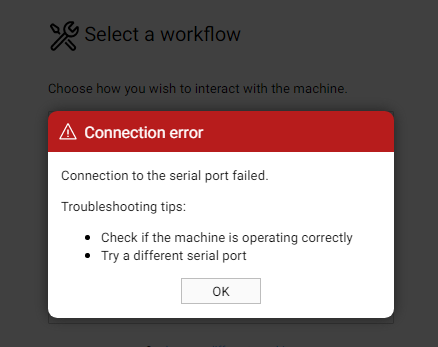
\includegraphics[width=0.6\textwidth]{connfailed}
        \caption{``Connection failed'' dialog.}
        \label{connfailed}
    \end{center}
\end{figure}

A status bar is displayed throughout the application. Its value is correctly
updated to match the current state of the connection (figure~\ref{status}).

\begin{figure}[ht]
    \begin{center}
        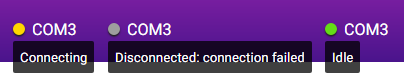
\includegraphics[width=0.6\textwidth]{status}
        \caption{Different values of the status bar.}
        \label{status}
    \end{center}
\end{figure}

\subsubsection{Command list and preview}

The command list component, displayed by every workflow screen, reflects the
state of the command queue. By attempting to send multiple long commands in a
row, the buffer overflow prevention mechanism discussed in section~\ref{sending}
may be observed.

The commands are displayed properly (figure~\ref{commandlist}). Their status is
shown to the right of the command text and they are color-coded. Errors may be
viewed by hovering over the ``Error'' label. The command list scrolls
automatically so that the currently executing command is always in the middle.

\begin{figure}[ht]
    \begin{center}
        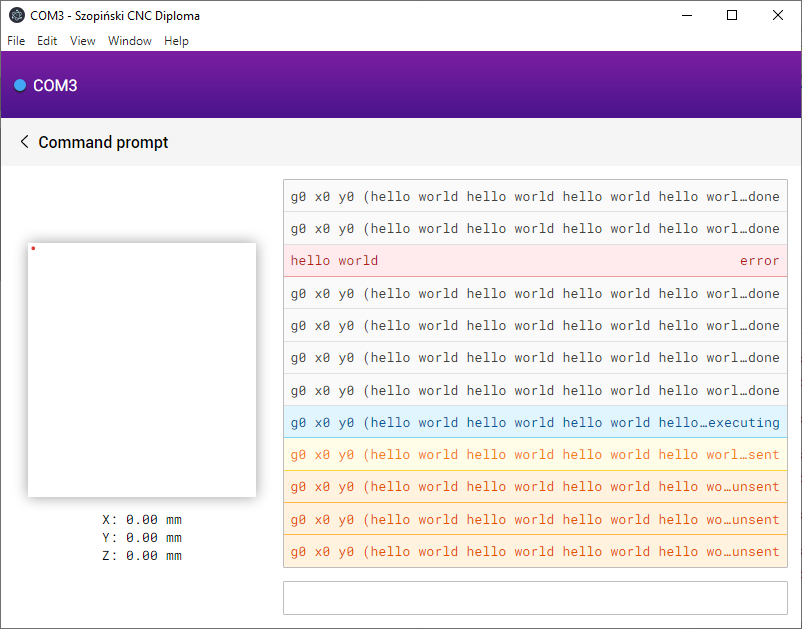
\includegraphics[width=0.6\textwidth]{commandlist}
        \caption{Command list showing commands at different lifecycle stages.}
        \label{commandlist}
    \end{center}
\end{figure}

\subsubsection{Bitmap tracing}
